\begin{enumerate}[\Large\bfseries 1.]

%-------------------1.
    \item \textbf{EJEMPLO DE INTEGRALES SABIENDO QUE LA FUNCIONES ES ESCALONADAS}

    \begin{enumerate}[\bfseries a)]

	%----------a.
	\item \textbf{(1.15 Ejercicio, problema 10. Tom Apostol, Calculus Vol 1)} Dado un entero positivo $p$. Una función escalonada $s$ está definida en el intervalo $[0,p]$ como sigue $s(x)=(-1)^n n$ si $x$ está en el intervalo $n\leq x < n+1$ siendo $n=0,1,2,...,p-1$; $s(p)=0$. Póngase $f(p)=\displaystyle\int_{0}^{p} s(x)\; dx.$\\\\

    \begin{enumerate}[\bfseries (a)]

	%----------(a)
	\item Calcular $f(3), f(4)$ y $f(f(3))$.\\\\
	    Respuesta.-\; Sea $$s(x) = \left\{ \begin{array}{lcl}
		(-1)^n n&si&n\leq x < n+1, \; n=0,1,...p-1\\
		\\0& si &x=p\\
	    \end{array}\right.$$
	    Entonces calculamos para $f(x)=\displaystyle\int_{0}^{p} s(x)\; dx$:
	    \begin{center}
	    \begin{tabular}{rclcrcr}
		$f(3)$ & $=$ & $\displaystyle\int_{0}^{3} s(x) \; dx$ & $=$ & $(-1)^0 0 (1-0) + (-1)\cdot 1\cdot(2-1) + (-1)^2 2 (3-2)$ & $=$ & $1$\\\\
		$f(4)$ & $=$ & $\displaystyle\int_{0}^{4} s(x) \; dx$ &$=$ & $\displaystyle\int_{0}^{3} s(x) \;dx + \int_{3}^{4} s(x) \; dx = 1 + (-1)^3 3 (4-3)$&$=$&$-2$\\\\
		$f(f(3))$&$=$&$f(1)$&$=$&$\displaystyle\int_{0}^{1} s(x) \; dx = (-1)^0 0 (1-0)$&$=$&$0$\\\\
	    \end{tabular}
	    \end{center}

	%----------(b)
	\item ¿Para qué valor o valores de $p$ es $|f(p)|=7$?\\\\
	    Respuesta.-\; Luego de completarlo por un bucle llegamos a la conclusión de que los números que cumplen la condición dada son $14,15$.\\\\

    \end{enumerate}

	%----------b)
	\item \textbf{Código fuente.}\\ 

	    \begin{enumerate}[\bfseries (a)]

		\item \lstinputlisting[language=Python]{python/tareas_mat/week1/func_ej1.15_prob10_a.py}
	    \vspace{2cm}

		\item \lstinputlisting[language=Python]{python/tareas_mat/week1/func_ej1.15_prob10_b.py}
	    \vspace{2cm}

	    \end{enumerate}
	
	%----------c)
	\item \textbf{Prueba de la ejecución del programa}.\\

	    \begin{enumerate}[\bfseries (a)]

	    \item .\\

		\begin{center}
		    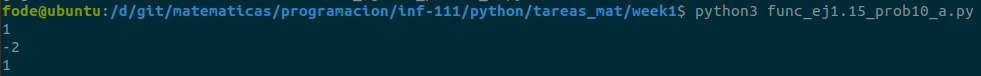
\includegraphics[scale=.45]{imagenes/tareas_mat/week1/func_ej1.15_prob10_a.png}
		\end{center}
	    
	    \item .\\
		\begin{center}
		    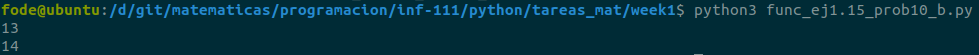
\includegraphics[scale=.45]{imagenes/tareas_mat/week1/func_ej1.15_prob10_b.png}
		\end{center}

	    \end{enumerate}

    \end{enumerate}

\newpage

%--------------------2.
\item \textbf{INTEGRAL DEFINIDA.}\\\\

    \begin{enumerate}[\bfseries a)]

	%----------a.
	\item \textbf{Teorema 1.13 (Tom Apostol, Calculus Vol. 1)} Supongamos $f$ creciente en un intervalo cerrado $[a,b]$. Sea $x_k = a + k(b-a)/n$ para $k=0,1,...,n$. Si $I$ es un número cualquiera que satisface las desigualdades $$\dfrac{b-a}{n}\sum\limits_{k=0}^{n-1} f(x_k)\leq I \leq \dfrac{b-a}{n}\sum\limits_{k=1}^n f(x_k) \qquad (2)$$
	para todo entero $n\geq 1$, entonces $I=\int_a^b f(x) \; dx$\\\\
	Demostración.-\; Sean $s_n$ y $t_n$ las funciones escalonadas de aproximación especial obtenidas por subdivisión del intervalo $[a,b]$ en $n$ partes iguales, como se hizo en la demostración del teorema 1.13. Entonces, las desigualdades (1.9) establecen que $$\int_a^b s_n \leq I \leq \int_a^b t_n$$
	para $n\geq 1$. Pero la integral $\int_a^b f(x) \; dx$ satisface las mismas desigualdades que $I$. Utilizando la igualdad $(1)$ tenemos $I\leq \int_a^b t_n$ \, como también \, $\int_a^b s_n \leq \int_a^b f(x) \; dx \quad \Longrightarrow\quad  - \int_a^b f(x) \; dx \leq -\int_a^b s_n$ entonces $$I-\int_a^b f(x)\; dx \leq \int_a^b t_n - \int_a^b s_n$$
	Similarmente usando las inecuaciones $\int_a^b s_n \leq I$ \, y \, $\int_a^b f(x) \; dx \leq \int_a^b t_n$ resulta que $$\int_a^b f(x) \; dx - I \leq \int_a^b t_n - \int_a^b s_n \quad \Longrightarrow \quad I - \int_a^b f(x) \; dx \geq - \left(\int_a^b t_n - \int_a^b s_n\right)$$ 
	Donde se concluye que $$0\leq \left| I - \int_a^b f(x) \; dx \right| \leq \int_a^b t_n - \int_a^b s_n = \dfrac{C}{n}$$
	par todo $n\geq 1$. Por consiguiente, según el teorema I.31, tenemos $I=\int_a^b f(x) \; dx$\\\\

	\newpage
	%----------b)
	\item \textbf{Código fuente.}\\ 
	    
	    \lstinputlisting[language=Python]{python/tareas_mat/week1/func_teorema1.13.py}
	    \vspace{3cm}
	
	%----------c)
	\item \textbf{Prueba de la ejecución del programa}.\\
	    \begin{center}
		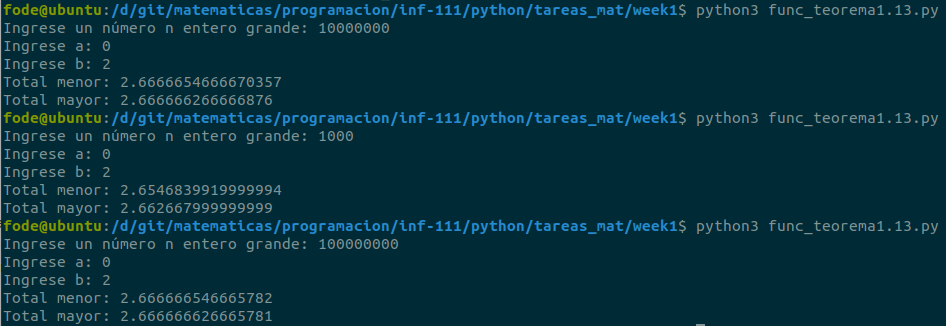
\includegraphics[scale=.5]{imagenes/tareas_mat/week1/1func_teorema1.13.png}
	    \end{center}

    \end{enumerate}

\newpage

%-------------------3.
\item \textbf{CÁLCULO DE LA INTEGRAL $\displaystyle\int_{o}^{b} x^p$ SIENDO $p$ ENTERO POSITIVO.}\\\\ 

    \begin{enumerate}[\bfseries a)]

	%----------a.
	\item \textbf{Teorema 1.15 (Tom Apostol, Calculus Vol. 1)} Si $p$ es un entero positivo y $b>0$, tenemos $$\int_0^b x^p \; dx = \dfrac{b^{p+1}}{p+1}$$\\
    Demostración.-\; Comencemos con las desigualdades $$\sum\limits_{k=1}^{n-1} k^p < \dfrac{n^{p+1}}{p+1}<\sum\limits_{k=1}^n k^p$$
    válidas para todo entero $n\geq 1$ y todo entero $p\geq 1$. Estas desigualdades se demostraron anteriormente. La multiplicación de esas desigualdades por $b^{p+1}/n^{p+1}$ nos da $$\dfrac{b}{n} \sum\limits_{k=1}^{n-1} \left(\dfrac{kb}{n}\right)^p<\dfrac{b^{p+1}}{p+1}<\dfrac{b}{n}\sum\limits_{k=1}^{n}\left(\dfrac{kb}{n}\right)^p$$
    Si ponemos, las desigualdades (2) del teorema 1.14 se satisfacen poniendo $f(x)=x^p, \;a=0$, entonces $I=\dfrac{b^{p+1}}{p+1}$. Resulta pues que $$\int_0^b x^p \; dx=\dfrac{b^{p+1}}{p+1}$$\\\\
    \vspace{1cm}

	%----------b)
	\item \textbf{Código fuente.}\\ 
	    
	    \lstinputlisting[language=Python]{python/tareas_mat/week1/func_teorema1.15.py}
	    \vspace{3cm}
	
	%----------c)
	\item \textbf{Prueba de la ejecución del programa}.\\
	    \begin{center}
		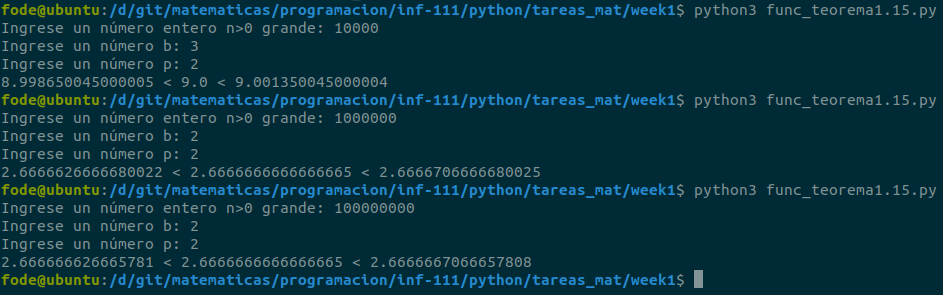
\includegraphics[scale=.47]{imagenes/tareas_mat/week1/func_teorema1.15.png}
	    \end{center}

    \end{enumerate}

\newpage

%--------------------4.
\item  \textbf{INTEGRACIÓN PARA EL SENO Y COSENO.}\\\\

    \begin{enumerate}[\bfseries a)]

	%----------a.
	\item \textbf{Teorema 2.4, Tom Apostol, Calculus Vol. 1} Si $0<a\leq \frac{1}{2}\pi,$ y $n\geq 1,$ tenemos $$\dfrac{a}{n}\sum_{k=1}^n \cos \dfrac{ka}{n}<\sen a < \dfrac{a}{n}\sum_{k=0}^{n-1} \cos \dfrac{ka}{n} \qquad \mbox{(2.6)}.$$
    Demostración.-\; Las desigualdades anterior serán deducidas de la identidad $$2\sen \dfrac{1}{2} x \sum_{k=1}^n \cos kx = \sen\left(n+\dfrac{1}{2}\right)x-\sen \dfrac{1}{2}x, \qquad \mbox{(2.7)}$$
    válida para $n\geq 1$ y todo real $x$. Para demostrar, utilizaremos las fórmulas de diferencias (g) del teorema 2.3 para poner $$2\sen\dfrac{1}{2}x\cos kx = \sen \left(k+\dfrac{1}{2}\right)x - \sen\left(k-\dfrac{1}{2}\right)x$$
    Haciendo $k=1,2,...,n$ y sumando esas igualdades, encontramos que en la suma del segundo miembro se reduce unos términos con otros obteniéndose (2.7).\\
    Si $\dfrac{1}{2}x$ no es un múltiplo entero de $\pi$ podemos dividir ambos miembros de (2.7) por $2\sen \dfrac{1}{2}x$ resultando $$\sum_{k=1}^n \cos kx = \dfrac{\sen(n+\frac{1}{2}x-\sen \frac{1}{2} x)}{2\sen \frac{1}{2}x}$$ 
    Reemplazando $n$ por $n-1$ y sumando $1$ a ambos miembros también obtenemos. (Ya que $\cos 0 = 1$).
    $$\sum_{k=0}^{n-1} \cos kx = \dfrac{\sen\left(n-\frac{1}{2}\right)x + \sen\frac{1}{2}x}{2\sen\frac{1}{2}x}$$
    Esas dos fórmulas son válidas si $x\neq2m\pi$, siendo $m$ entero. Tomando $x=a/n$, donde $0<a<\frac{1}{2}\pi$ encontramos que el par de desigualdades (2.6) es equivalente al siguiente 
    $$\dfrac{a}{n}\dfrac{\sen\left(n+\dfrac{1}{2}\right)\dfrac{a}{n} - \sen \left(\dfrac{a}{2n}\right)}{2\sen\left(\dfrac{a}{2n}\right)} < \sen a < \dfrac{a}{n}\dfrac{\sen\left(n-\dfrac{1}{2}\right)\dfrac{a}{b}+\sen\left(\dfrac{a}{2n}\right)}{2\sen\left(\dfrac{a}{2n}\right)}$$
    Este par, a su vez es equivalente al par
    $$\sen\left(n+\dfrac{1}{2}\right)\dfrac{a}{n}-\sen\left(\dfrac{a}{2n}\right) < \dfrac{\sen\left(\dfrac{a}{2n}\right)}{\left(\dfrac{a}{2n}\right)} \sen a < \sen\left(n-\dfrac{1}{2}\right)\dfrac{a}{n}+\sen\left(\dfrac{a}{2n}\right) \qquad \mbox{(2.8)}$$
    Por consiguiente demostrar (2.6) equivale a demostrar (2.8). Demostraremos que se tiene 
    $$\sen\left(2n+1\right)\theta -\sen \theta < \dfrac{\sen \theta}{\theta} < \sen(2n-1)\theta +\sen \theta \qquad \mbox{(2.9)}$$
    para $0<2n\theta\leq \frac{1}{2}\pi$. Cuando $\theta = a/(2n)$ (2.9) se reduce a (2.8).\\
    Para demostrar la desigualdad de la parte izquierda de (2.9), usamos la fórmula de adición para el seno poniendo $$\sen(2n+1)\theta = \sen 2n\theta \cos \theta + \cos 2n\theta \sen \theta < \sen 2n\theta \dfrac{\sen \theta}{\theta} + \sen \theta,$$
    habiendo usado también las desigualdades $$\cos \theta < \dfrac{\sen \theta}{\theta}, \quad 0z<\cos 2n\theta \leq 1, \quad \sen \theta > 0, \qquad \mbox{(2.10)}$$
    siendo todas válidas ya que $0<2n\theta \leq \frac{1}{2}\pi$. La desigualdad (2.10) equivale a la parte izquierda de (2.9).\\
    Para demostrar la parte derecha de (2.9), utilizamos nuevamente la fórmula de adición para el seno poniendo $$\sen(2n-1)\theta = \sen 2n\theta \cos \theta - \cos 2n\theta \sen \theta$$
    Sumando $\sen \theta$ ambos miembros, obtenemos $$\sen(2n-1)\theta + \sen \theta = \sen 2n\theta \left(\cos \theta +\sen \theta \dfrac{1-\cos 2n\theta}{\sen 2n\theta}\right) \qquad \mbox{(2.11)}$$
    Pero ya que tenemos $$\dfrac{1-\cos 2n\theta}{\sen2n\theta}=\dfrac{2\sen^2n\theta}{2\sen n\theta \cos n \theta}=\dfrac{\sen n\theta}{\cos n \theta}$$
    el segundo miembro de (2.11) es igual a $$\sen 2n\theta \left(\cos \theta + \sen \theta \dfrac{\sen n \theta}{\cos n\theta}\right) = \sen 2 n\theta \dfrac{\cos \theta \cos n\theta + \sen \theta \sen n \theta}{\cos n \theta} = \sen 2n\theta \dfrac{\cos (n-1) \theta}{\cos n \theta}$$
    Por consiguiente, para completar la demostración de (2.9), necesitamos tan sólo demostrar que 
    $$\dfrac{\cos(n-1)\theta}{\cos n\theta}>\dfrac{\sen \theta}{\theta} \qquad \mbox{(2.12)}$$
    Pero tenemos $$\cos n\theta = \cos(n-1)\cos theta - \sen(n-1)\theta \sen \theta < \cos(n-1)\theta \cos \theta < \cos(n-1)\theta \dfrac{\theta}{\sen \theta},$$
    en donde otra vez hemos utiliado la desigualdad fundamental $\cos \theta < \theta/sen \theta.$ ya que $\left(\cos x < \dfrac{x}{\sen x}\right)$, esta último relación implica (2.12), con lo que se completa la demostración del teorema 2.4.\\\\

	%----------b)
	\item \textbf{Código fuente.}\\ 
	    
	    \lstinputlisting[language=Python]{python/tareas_mat/week1/func_teorema2.4.py}
	    \vspace{3cm}
	
	%----------c)
	\item \textbf{Prueba de la ejecución del programa}.\\
	    \begin{center}
		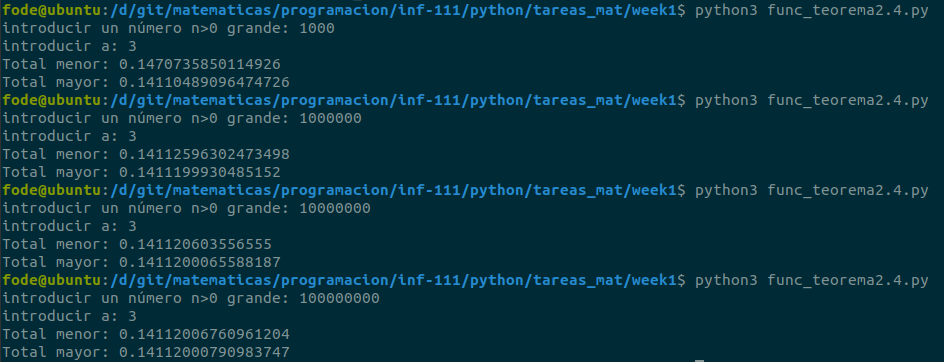
\includegraphics[scale=.5]{imagenes/tareas_mat/week1/func_teorema2.4.png}
	    \end{center}

    \end{enumerate}

\newpage


%-------------------5.
\item \textbf{INTEGRACIÓN PARA SENO Y COSENO GENERALIZADO.}\\\\

    \begin{enumerate}[\bfseries a)]

	%----------a.
	\item \textbf{Teorema 2.5, Tom Apostol, Calculus Vol. 1} Si dos funciones $\sen$ y $\cos$ satisfacen las propiedades fundamentales de la 1 a la 4, para todo $a$ real se tiene $$\int_0^a \cos x\; dx = \sen a, \qquad \mbox{(2.13)}$$ $$\int_0^a x\; dx = 1-\cos a. \qquad \mbox{(2.14)}$$\\
    Demostración.-\; Primero se demuestra (2.13), y luego usamos (2.13) para deducir (2.14). Supongamos que $0<a\leq \frac{1}{2}\pi$. Ya que el coseno es decreciente en $[0,a]$ podemos aplicar el teorema 1.14 y las desigualdades del teorema 2.4 obteniendo (2.13). La fórmula es valida también para $a=0$, ya que ambos miembros son cero. Pueden ahora  utilizarse las propiedades de la integral para ampliar su validez todos los valores reales $a$.\\
    Por ejemplo, si $-\frac{1}{2}\pi \leq a \leq 0$, entonces $0\leq -a\leq \frac{1}{2}\pi$, y la propiedad de reflexión nos da $$\int_0^a \cos x\; dx = -\int_0^{-a} \cos (-x) \; dx = - \int_0^{-a} \cos x \; dx = -\sen (-a) = \sen a.$$
    Así, pues, (2.13) es válida en el intervalo $\left[-\frac{1}{2}\pi,\frac{1}{2}\pi\right]$. Supongamos ahora que $\frac{1}{2}\pi \leq a \leq \frac{3}{2}\pi$. Entonces $-\frac{1}{2}\pi\leq a-\pi\leq \frac{1}{2}\pi$, de modo que $$\int_0^a \cos x \; dx = \int_{0}^{\pi/2} \cos x \; dx + \int_{\pi/2}^a \cos x \; dx = \sen\frac{1}{2}\pi + \int_{-\pi/2}^{a-\pi} \cos(x+\pi)\; dx = 1-\int_{-\pi/2}^{a-\pi} \cos x \; dx = $$ $$=1 - \sen(a-\pi) + \sen\left(-\frac{1}{2}\pi\right) = \sen a$$
    Con ellos resulta que (2.13) es válida para todo $a$ en el intervalo $\left[-\frac{1}{2}\pi,\frac{3}{2}\pi\right]$. Pero este intervalo tiene longitud $2\pi$, con lo que la fórmula (2.13) es válida para todo $a$ puesto que ambos miembros son periódicos respecto a $a$ con período $2\pi$\\
    Seguidamente usamos (2.13) para deducir (2.14). Ante todo demostramos que (2.14) es válida cuando $a=\pi/2$. Aplicando sucesivamente, la propiedad de traslación, la co-relación $\sen\left(x+\frac{1}{2}\pi\right)$, y la propiedad de reflexión, encontramos 
    $$\int_0^{\pi/2}\sen x\; dx = \int_{-\pi/2}^0 \sen \left(x+\dfrac{\pi}{2}\right)\; dx = \int_{-\pi/2}^0 \cos x \; dx = \int_0^{\pi/2}\cos (-x) \; dx$$
    Haciendo uso de la relación $\cos(-x)=\cos x$ y la igualdad (2.13), se obtiene $$\int_0^{\pi/2}\sen x\; dx = 1$$
    Por consiguiente, para cualquier $a$ real, podemos escribir $$\int_0^a \sen x\;dx = \int_0^{\pi/2} \sen x\; dx + \int_{\pi/2}^a \sen x \; dx = 1 + \int_0^{a-\pi/2}\sen \left(x+\dfrac{\pi}{2}\right)\; dx =$$ $$= 1+\int_0^{a-\pi/2} \cos x \; dx = 1+\sen\left(a-\dfrac{\pi}{2}\right) = 1-\cos a$$
    Esto demuestra que la igualdad (2.13) implica (2.14).\\\\

    Usando (2.13) y (2.14) junto con la propiedad aditiva $$\int_a^b f(x) \; dx = \int_0^b f(x)\; dx - \int_0^a f(x)\; dx $$
    llegamos a las fórmulas de integración más generales
    $$\int_a^b \cos x \; dx = \sen b - \sen a$$
	y $$\int_a^b \sen x \; dx = (1-\cos b) - (1-\cos a) = -(\cos b - \cos a).$$
	Si nuevamente utilizamos el símbolo especial $f(x)\left|_a^b\right.$ para indicar la diferencia $f(b)-f(a)$, podemos escribir esas fórmulas de integración en la forma 
	$$\int_a^b \cos x \;dx = \sen x \bigg|_a^b \qquad y \qquad \int_a^b \sen x\; dx = -\cos x \bigg|_a^b$$

	Con los resultados del ejemplo 1 y la propiedad de dilatación $$\int_a^b f(x)\; dx = \dfrac{1}{c}\int_{ca}^{cb} f(x/c)\; dx,$$
	obtenemos las fórmulas siguientes, válidas para $c\neq 0$;
	$$\int_a^b \cos cx \; dx = \dfrac{1}{c}\int_{ca}^{cb} \cos x \; dx = \dfrac{1}{c}(\sen cb - \sen ca)$$
	y $$\int_a^b \sen cx \; dx = \dfrac{1}{c} \int_{ca}^{cb} \sen x \; dx = -\dfrac{1}{c}(\cos cb -\cos ca).$$

	La identidad $\cos 2x = 1-2\sen^2 x$ implica $\sen^2 x = \frac{1}{2}(1-\cos 2x)$ con lo que, a partir del ejemplo 2, obtenemos $$\int_a^b \sen^2 x \; dx = \dfrac{1}{2}\int_0^a (1-\cos 2x)\; dx = \dfrac{a}{2}-\dfrac{1}{4}\sen 2a$$
	Puesto que $\sen^2 x + \cos^2 x = 1,$ encontramos también $$\int_0^a \cos^2 x \; dx = \int_0^a(1-\sen^2 x)\; dx = a - \int_0^a \sen^2 x\; dx = \dfrac{a}{2}+\dfrac{1}{4}\sen 2a$$
	
	\newpage
	%----------b)
	\item \textbf{Código fuente.}\\ 
	    
	    \lstinputlisting[language=Python]{python/tareas_mat/week1/func_teorema2.5.py}
	    \vspace{3cm}
	
	%----------c)
	\item \textbf{Prueba de la ejecución del programa}.\\
	    \begin{center}
		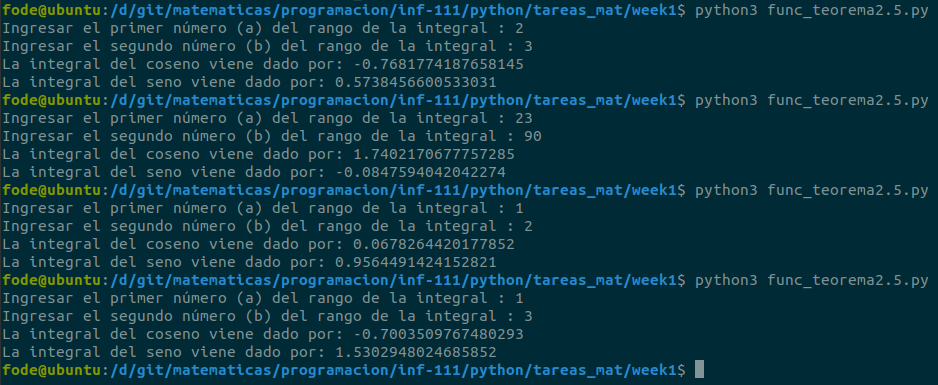
\includegraphics[scale=.47]{imagenes/tareas_mat/week1/func_teorema2.5.png}
	    \end{center}

    \end{enumerate}

\newpage




\end{enumerate}
